\documentclass[sigconf, fleqn, prologue, dvipsnames]{acmart}
\usepackage{booktabs}
\usepackage{placeins}
% \usepackage{algorithmicx}
% \usepackage[noend]{algpseudocode}
% \usepackage{algorithm}
\usepackage[ruled, procnumbered]{algorithm2e}
\usepackage{subcaption}


%% \BibTeX command to typeset BibTeX logo in the docs
\AtBeginDocument{%
  \providecommand\BibTeX{{%
    \normalfont B\kern-0.5em{\scshape i\kern-0.25em b}\kern-0.8em\TeX}}}

%% These commands are for a PROCEEDINGS abstract or paper.
\settopmatter{printacmref=false} % Removes citation information below abstract
\renewcommand\footnotetextcopyrightpermission[1]{} % removes footnote with conference information in 

\acmConference[GM LAB]{Graphical Models LAB}{August 9}{Jena, Germany}


\graphicspath{{graphics/}}

\definecolor{myblue}{RGB}{46, 59, 160}
\hypersetup{
    pdfstartpage=1,
    pdfstartview = FitB,
    pdfpagelayout=SinglePage,
    pdftitle={Project Report},
    pdfsubject={Structure Learning},
    pdfauthor={Maurice Wenig},
    pdfcreator={Maurice Wenig},
    pdfproducer={Maurice Wenig},
    pdfkeywords={meta, information, pdf, hyperref, latex},
    colorlinks=true,
    linkcolor=myblue,
    citecolor=myblue
}

%----- algorithm2e
\SetKwInOut{Input}{input}
\SetKwInOut{Output}{output}

%----- new commands
\newcommand{\Romannumeral}[1]{\MakeUppercase{\romannumeral #1}}
\newcommand{\set}[1]{\{#1\}}
\newcommand{\abs}[1]{\left\vert #1 \right\vert}
\newcommand{\norm}[1]{\left\| #1 \right\|}
\newcommand{\skal}[2]{\left\langle #1 | #2 \right\rangle}
\newcommand{\numberthis}{\addtocounter{equation}{1}\tag{\theequation}}
\newcommand{\maybe}[1]{%
	\textcolor{Goldenrod}{#1?}%
    \reversemarginpar%
    \marginpar{\raggedleft\textcolor{Goldenrod}{\rule{2mm}{2mm}}}%
}
%----- defs
\def\notiff{\mathrel{{\ooalign{\hidewidth$\not\phantom{"}$\hidewidth\cr$\iff$}}}}
\def\R{\mathbb{R}}
\def\bbone{\text{\usefont{U}{bbold}{m}{n}1}}
\def\1{\mathbb{1}}
\def\O{\mathcal{O}}
\def\T{\top}
\def\pa{\text{pa}}
\def\ndy{%
    % \textcolor{red} {\hfill not done yet!}
    \reversemarginpar%
    \marginpar{\raggedleft\textcolor{red}{\rule{2mm}{2mm}}}%
}
\def\ghostline{\hfill\vspace*{-5mm}}

%----- main
\begin{document}
\title[Project Report]{Project Report\\\large Graphical Models LAB}
\author{Maurice Wenig}
\affiliation{%
	\institution{Friedrich Schiller University Jena}
	\country{Germany}%
}
\email{maurice.wenig@uni-jena.de}

\maketitle
% \let\thefootnote\relax\footnotetext{AEPRO 2022, March 1, Jena, Germany. Copyright \copyright 2022 for this paper by its authors. Use permitted under Creative Commons License Attribution 4.0 International (CC BY 4.0).}


\section{Introduction}
Learning graphical models is a big aspect of machine learning.
But for the parameters of the model to be learned, it is often assumed that the structure is already given, which includes information about dependencies and independencies between features.
However in practice, that is not the case.
Sometimes even the opposite might be true, that the structure between features itself is much more relevant than the actual amplitude of their interactions, with the hope of being able to interpret the interactions (e.g. in a causal context).
This is also an inspiration for our assignment, where our main task is coming up with a search strategy to find a sparse Bayesian Network that fits the data we were given.

For our assignment, we focused on Gaussian Bayesian Networks (GBN).
A GBN is a Bayesian Network where the conditional distributions of a feature given their parents is a Gaussian.
Another constraint to the GBN is that the mean paramater of the Gaussian, that is the conditional distribution, can only depend linearly on the values of the feature's parents in the Network Graph.
So with $n$ as the total number of features, the problem of learning the distribution $p(x_i | x_{\pa(i)})$ for a feature $i \in [n]$, its value $x_i \in \R$, and the value of their parents $x_{\pa(i)} \in \R^{n_i}$ is equivalent to learning $\hat{\beta_i}^* \in \R, \hat{\beta_i} \in \R^{n_i}, \hat{\sigma_i} \in \R$ such that $p(x_i | x_{\pa(i)}) \sim \mathcal{N}(\hat{\beta_i}^* + \hat{\beta_i}^\T x_{\pa(i)}, \hat{\sigma_i}^2)$.
Now for these parameters, the ML-estimates have a simple closed-form solution (it is just linear regression), so finding the best parameters for any given structure is simple and efficient.

% https://doi.org/10.1016/j.dss.2009.05.016
The dataset we were given spans different attributes of Portuguese "Vinho Verde" wine, which was originally used in [cite\ndy].
It consists of twelve features: eleven continuous physicochemical attributes and one discrete sensory attribute (quality).
Here, i will treat quality as a continuous feature.

\maybe{visualize data}
\FloatBarrier


\section{Methods}
% talk about what greedy search algorithm was used (in the overview paper (citation?) they said that it's rather common and well performing, so i chose the greedy algorithm (special case hill climbing with tabu walks and restarts))
% present the hill climbing algorithm (attention! details needed how tabu walks and random restarts are combined! this is not mentioned in the overview)
% -> maybe reasoning needed as to why tabu walks and the random restarts were combined in this way.
For the structure learning algorithm, i implemented a tabu search, because it generally performs well in accuracy and runtime (cite overview\ndy).
I also combined the tabu search with random restarts. The entire parameterized algorithm is illustrated in \autoref{algo:methods:search}.
It is important to note that the function arguments are all passed by reference, so mutations inside of functions will affect the passed argument even outside the function.

\begin{algorithm}
	\caption{Tabu Search with Random Restarts}
	\label{algo:methods:search}
	\Input{dataset $D$, initial DAG $G$}

	$G_{max} \gets \text{copy of } G$\;
	HillClimb($D, G_{max}$)\;
	\For{$t_0$ times}{
		TabuWalk($D, G_{max}, s_0, l$)\;
		HillClimb($D, G_{max}$)\;
	}
	\For{$t_1$ times}{
		RandomRestart($D, G_{max}, s_1$)\;
		HillClimb($D, G_{max}$)\;
		\For{$t_0$ times}{
			TabuWalk($D, G_{max}, s_0, l$)\;
			HillClimb($D, G_{max}$)\;
		}
	}
\end{algorithm}

First we do a hill climb. After the first hill climb, we do $t_0$ tabu walks followed by another hill climb each.
Then we do a random restart and do it all again. The random restart procedure is repeated $t_1$ times.
\begin{itemize}
	\item $t_0$: number of tabu walks
	\item $s_0$: maximum number of steps of a tabu walk
	\item $l$: length of the tabu list
	\item $t_1$: number of random restarts
	\item $s_1$: number of random steps during a random restart
\end{itemize}

\FloatBarrier


\subsection{Hill Climbing}
% talk about how you climb the hill (how do you find all of the possible changes at any given point? (you need to check for cycles etc. - how do you do that efficiently (cite the guy)))
% how do you efficiently evaluate the change? (you never copy, the adjacency matrix, but apply the change, see what happens, and revert it)
% how do you evaluate if one change is better than another efficiently? (you never re-calculate the whole objective function, because the changes can be evaluated locally)
% ^ this is further discussed in [Implications for Hill Climbing]
In every iteration, the hill climbing algorithm computes the best possible elementary change among all changes.
If this change improves the objective function, it is applied.
This algorithm is illustrated in \autoref{func:methods:climb_hill}.

\begin{function}
	\caption{ClimbHill()}
	\label{func:methods:climb_hill}
	\Input{dataset $D$, current DAG $G$}
	\While{$S_{max}$ increases}{
		$S_G \gets Score(G, D)$\;
		$c_{max} \gets$ IMPOSSIBLY\_BAD\_CHANGE\;
		$C \gets AllChanges(G)$\;
		\ForEach{$c \in C$}{
			apply the change $c$ to $G$\;
			$S_c \gets Score(G, D)$\;
			undo the change $c$ in $G$\;
			\uIf{$S_c > S_{max}$}{
				$S_{max} \gets S_c$\;
				$c_{max} \gets c$\;
			}
		}
		\uIf{$S_c > S_G$}{
			apply the change $c_{max}$ to $G$\;
		}
	}
\end{function}

In order to avoid copying the adjacency matrix every time a change is applied, the adjacency matrix is changed in-place, and then the score is evaluated.
This is also improves the efficiency of generating all possible changes, which is illustrated in \autoref{func:methods:all_changes}.
The evaluation of the score can be sped up by only evaluating local changes of the changed nodes.
This is further discussed in \autoref{sec:methods:score:implications}.

\begin{function}
	\caption{AllChanges($G$)}
	\label{func:methods:all_changes}
	\Input{DAG $G$}
	\Output{all possible changes to $G$ such that $G$ is still a DAG after the application of the change}
	$C \gets \emptyset$\;
	\ForEach{$(u,v) \in E_G$}{
		$c \gets \text{FLIP}(u, v)$\;
		apply the change $c$ to $G$\;
		\uIf{$G$ does not have a cycle}{
			$C \gets C \cup \set{c}$\;
		}
		undo the change $c$ in $G$\;
	}
	\ForEach{$(u,v) \in E_G$}{
		$c \gets \text{DELETION}(u, v)$\;
		\tcp{deletions do not add cycles}
		$C \gets C \cup \set{c}$\;
	}
	$G^t \gets$ TransitiveClosure($G$)\;
	\ForEach{$u,v \in V_G, u \neq v$}{
		\uIf{$(u,v) \notin E_G$ and $(v,u) \notin E_{G^t}$}{
			$c \gets \text{ADDITION}(u, v)$\;
			$C \gets C \cup \set{c}$\;
		}
	}
	\Return{$C$}
\end{function}

Another key point to the efficiency of \autoref{func:methods:all_changes} is the efficiency of the cyclicity check.
For additions, this can be done by computing the transitive closure $G^t$ of $G$, which can be done in $\O(\abs{V_G}^3)$.
Then if $(v, u) \notin E_{G^t}$, the addition of $(u,v)$ will not create a new cycle.
For flips, i didn't find a more efficient way than completely checking the resulting graph for cycles.
This can be done in $\O(\abs{V_G} + \abs{E_G})$ with Kosaraju-Sharir's algorithm [cite\ndy].
But because we use ajdacency matrices instead of adjacency lists, Kosaraju-Sharir's algorithm takes $\O(\abs{V_G}^2)$.
Therefore, the resulting time for generating all flips is $\O(\abs{E_G} \cdot \abs{V_G}^2)$.
It follows that the overall time for generating all possible changes is $\O((\abs{V_G} + \abs{E_G}) \cdot \abs{V_G}^2)$.

\FloatBarrier


\subsection{Tabu Walks}
% talk about how you keep the tabu list efficient
% you hash the adjacency matrix to compressed byte arrays instead of saving 2-dimensional bitstrings and put em in the queue
% then at tabu walk start you put them all into set, this allows you to efficiently compute all changes that are not in the tabu lists, because lookups in the hash set are efficient. (and the number of changes you have to check is huge, so this should save a lot of time)
% maybe say that it uses the same algorithm for finding the best change out of a set of changes as the hill climbing algorithm, just that the set of changes passed is now different (non-tabu changes instead of all possible changes)
For the tabu walks, we use a FiFo-Queue that keeps track of hashes of each visited adjacency matrix. This queue is called the tabu list.
The rest of the algorithm is very similar to hill climbing, just with minimal adjustments:
\begin{itemize}
	\item changes that result in visited adjacency matrices are not considered
	\item in each iteration, the top change is applied, disregarding whether it improves the objective function
	\item if the current value of the objective function exceeds the initial value of the objective function, the tabu walk is stopped
\end{itemize}
To efficiently check which changes result in visited adjacency matrices, a counter with the number of occurencces in the tabu list for each hash is used.
This counter can efficiently be updated whenever hashes of adjacency matrix are appended to or removed from the queue.


\subsection{Random Restarts}
% sometimes we just do random changes, maybe talk about your choice of uniform distribution among all possible changes (so we don't have a bias)
% maybe talk about how a bias might be introduced to prioritize additions and deletions, or maybe prioritize flips, idk might be interesting.
% priors for the random walk could be studied in future works. (maybe find out if someone already did that? cite them if someone exists -> like here, they tried but i won't get into it. if you wanna know more about it, check em out)
For the random restarts, a list of all possible changes is generated at each step.
Then one of them is chosen from a uniform distribution.


\subsection{Choice of Optimized Score}
% TODO: rewrite this? this is just for remembering what i did and why
For the score function $p(G | D) \propto p(D | G) \cdot p(G)$, i used the approximation
\begin{align*}
	p(D | G)     & \approx p(D | G, \hat{\theta})               \\
	\hat{\theta} & := \arg\max\limits_{\theta} p(D | G, \theta)
\end{align*}
and the prior
$$p(G) \propto \frac{1}{|E|^\lambda}$$
With this, the objective function can be decomposed into the sum of independent node scores and a regularization term.
\begin{align*}
	\arg\max\limits_G p(G | D) & = \arg\max\limits_G \log p(D | G) + \log p(G)                             \\
	                           & \approx \arg\max\limits_G \log p(D | G, \hat{\theta}) - \lambda \abs{E_G} \\
	                           & = \arg\max\limits_G \sum\limits_{i \in [n]} S_i(G) - \lambda \abs{E_G}
\end{align*}
where
$$S_i(G) := -\abs{D} \cdot \log \hat{\sigma_i} - \frac{1}{2} \sum\limits_{x \in D} \left(\frac{x_i - (\hat{\beta_i}^\T x_{\pa(i)} + \hat{\beta_i}^*)}{\hat{\sigma_i}}\right)^2$$
and $\hat{\theta} := \left(\hat{\beta_i}, \hat{\beta_i}^*, \hat{\sigma_i}\right)_{i \in [n]}$ are the respective ML estimates for
$$p(x_i | x_{\pa(i)}) \sim \mathcal{N}(\hat{\beta_i}^\T x_{\pa(i)} + \hat{\beta_i}^*, \sigma_i^2)$$
A derivation of this can be found in \autoref{sec:calc:score_function}.

\subsubsection{Implications for Hill Climbing}
\label{sec:methods:score:implications}
Elementary changes (addition, substraction, flip of an edge) only influence local distributions.
That means if we construct a graph $G'$, where $G'$ was made by applying an elementary change to an edge $(u, v)$ in $G$, the comparison $p(G' | D) > p(G | D)$ can be evaluated locally:
\begin{align*}
	\sum\limits_{i \in [n]} S_i(G') - \lambda \abs{E_{G'}}                               & > \sum\limits_{i \in [n]} S_i(G) - \lambda \abs{E_{G}}                  \\
	\iff\sum\limits_{i \in [n]} S_i(G') - S_i(G)                                         & > \lambda (\abs{E_{G'}} - \abs{E_{G}})                                  \\
	\iff\underbrace{\sum\limits_{i \in \set{u,v}} S_i(G') - S_i(G)}_{:= \Delta_S(G', G)} & > \lambda \underbrace{(\abs{E_{G'}} - \abs{E_{G}})}_{:= \Delta_E(G',G)}
\end{align*}
Where the second equivalence holds because $S_i(G)$ only depends on node $i$ and its parents.
Therefore $S_i(G') = S_i(G)$ for $i \notin \set{u, v}$.
Note that $\Delta_E(G',G)$ only depends on the type of change applied to $G$:
$$
	\Delta_E(G',G) = \begin{cases}
		1  & \text{addition} \\
		0  & \text{flip}     \\
		-1 & \text{deletion} \\
	\end{cases}
$$
$\Delta_S(G', G)$ measures the improvement of node scores when the change is applied to $G$.

Similarly, two alterations $G_1$ and $G_2$ of $G$ can be compared:
\begin{align*}
	\sum\limits_{i \in [n]} S_i(G_1) - \lambda \abs{E_{G_1}} & > \sum\limits_{i \in [n]} S_i(G_2) - \lambda \abs{E_{G_2}} \\
	\iff \Delta_S(G_1, G) - \Delta_S(G_2, G)                 & > \lambda \left(\Delta_E(G_1,G) - \Delta_E(G_2,G)\right)   \\
\end{align*}
A derivation of this can be found in \autoref{sec:calc:comparison}.

The interpretation of this is that a change has to bring an improvement of at least $\lambda$ per edge in order to improve the whole objective function (which makes sense looking at the objective function).
But more importantly, this allow a very efficient comparison of two different changes, which we need to efficiently find the best possible change for hill climbing and tabu walks.
\FloatBarrier

\subsection{Parameter Fine-Tuning}
% how did you fine tune the parameters? what are we looking for? (for the tabu walk and the random restarts to actually climb out of local optima and result in better optima)
% include your funny little plots here
The parameters with the highest impact on the outcome are $\lambda$ (in the objective function), $s_0$ (length of the tabu walks), and $s_1$ (length of the random walks).
The impact of $\lambda$ will be analyzed in \autoref{sec:results:structures}.
With $s_0$ and $s_1$, we can fine tune the ability to walk out of slim local maxima, and stay in wider maxima.
In order to do this, we can analyze the score history over time after the first hill climb.

In \autoref{fig:methods:fine_tuning}, we look at two examples of a score history where the parameters still need some tuning.
In \autoref{fig:methods:fine_tuning:too_short_t} the tabu walks do not manage to escape slim maxima, because tabu walks are too short.
In \autoref{fig:methods:fine_tuning:too_long_r} the random restarts distort the top adjacency matrix too much and return to worse local maxima, because the random walks are too long.

\begin{figure}
	\centering
	\begin{subfigure}{0.2\textwidth}
		\centering
		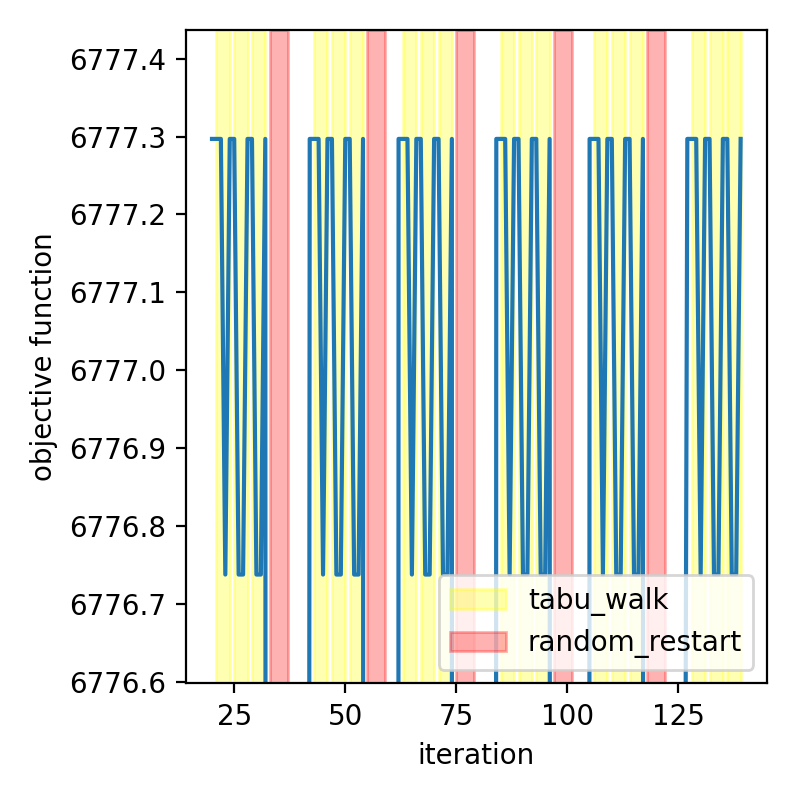
\includegraphics[scale=0.35]{graphics/tabu_small_2ts.png}
		\caption{Short tabu walks}
		\label{fig:methods:fine_tuning:too_short_t}
	\end{subfigure}
	\begin{subfigure}{0.2\textwidth}
		\centering
		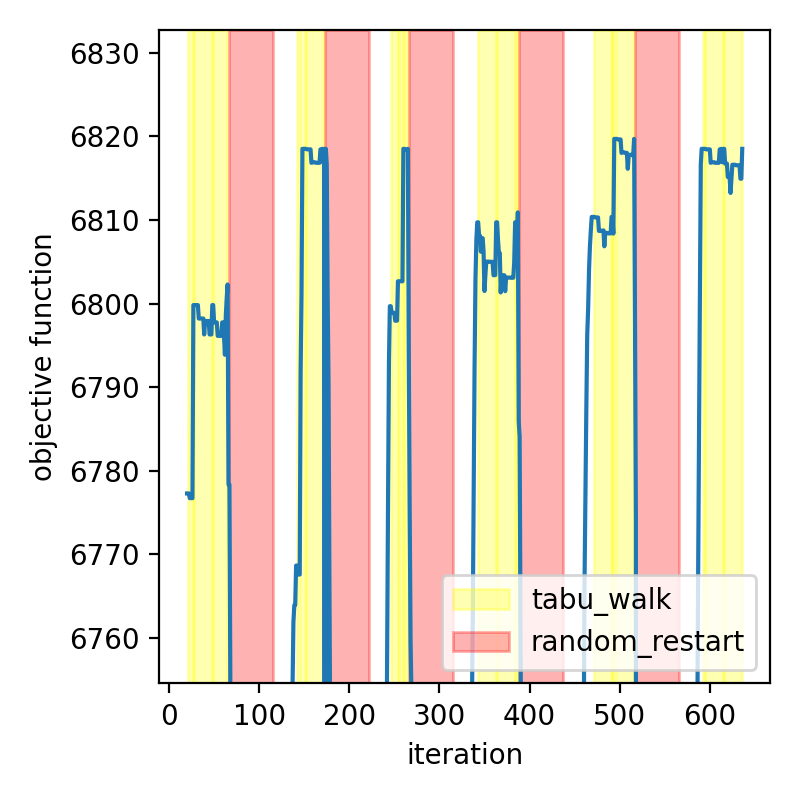
\includegraphics[scale=0.35]{graphics/tabu_small_2tr.png}
		\caption{Long random walks}
		\label{fig:methods:fine_tuning:too_long_r}
	\end{subfigure}
	\caption{Score history after the first hill climb}
	\label{fig:methods:fine_tuning}
\end{figure}
\FloatBarrier


\subsection{Analysis}
\subsubsection{Parameterization}
\label{sec:methods:analysis:parameterization}
For all measurements, i parameterized the greedy search in three in different ways for different numbers of expected parameters (see \autoref{tab:methods:parameters}).

\begin{table}[htbp]
	\caption{Parameterization of the greedy search}
	\label{tab:methods:parameters}
	\begin{tabular}{llccccc}
		\toprule
		Parameterization & $\lambda$     & $t_0$ & $s_0$ & $m$  & $t_1$ & $s_1$ \\
		\midrule
		big              & 0 - 3         & 3     & 150   & 2000 & 5     & 10    \\
		medium           & 3 - 25        & 3     & 80    & 400  & 5     & 5     \\
		small            & 25 - $\infty$ & 3     & 20    & 100  & 5     & 5     \\
		\bottomrule
	\end{tabular}
\end{table}

\subsubsection{Likelihood}
In order to measure the likelihood of the generated structures, i split up the data we were given into a training set and a test set.
I trained the models with different $\lambda$ on the train set to generate the adjacency matrices.
Then i used cross validation on the test set to measure the likelihood of the ML-estimate of the parameters for each adjacency matrix.

\subsubsection{Performance}
While generating the structures with my train set, i also measured the runtime of the greedy search.
The specifications of the machine the time was measured on can be found in [APPENDIX\ndy].

\subsubsection{Submissions}
We were also given a submission site where we could anonymously upload our adjacency matrices and see how we compare to others.
The submission site computes the likelihood of our submitted adjacency matrices with a secret test set.

\subsubsection{Parameterization Comparison}
For the comparison of the small parameterization with the other two, i measured the likelihoods and runtimes on the same train and test sets, on the same machine, but on different days.
For this reason, the runtime of the smaller models in its intended $\lambda$-region is included in the results section.


\section{Results}
\subsection{Generated Structures}
\label{sec:results:structures}
% refer to some generated graphs for different lambdas that are visualized in the appendix
% idk look at the graphs and maybe there's something to note?
% yes there def is: how sparse is a graph for a given lambda? -> include the plot
The greedy search generates different structures depending on the regularization constant $\lambda$ in the objective function.
The number of paramaters in the generated structures is $\#params = 2 \abs{V_G} + \abs{E_G}$ for any structure $G$.
Because of the relationship between edge importance and $\lambda$ discussed in \autoref{sec:methods:score:implications}, this term is expected to decrease as $\lambda$ increases.
This was confirmed in practice. The results are illustrated in \autoref{fig:results:n_params}.
\begin{figure}
	\centering
	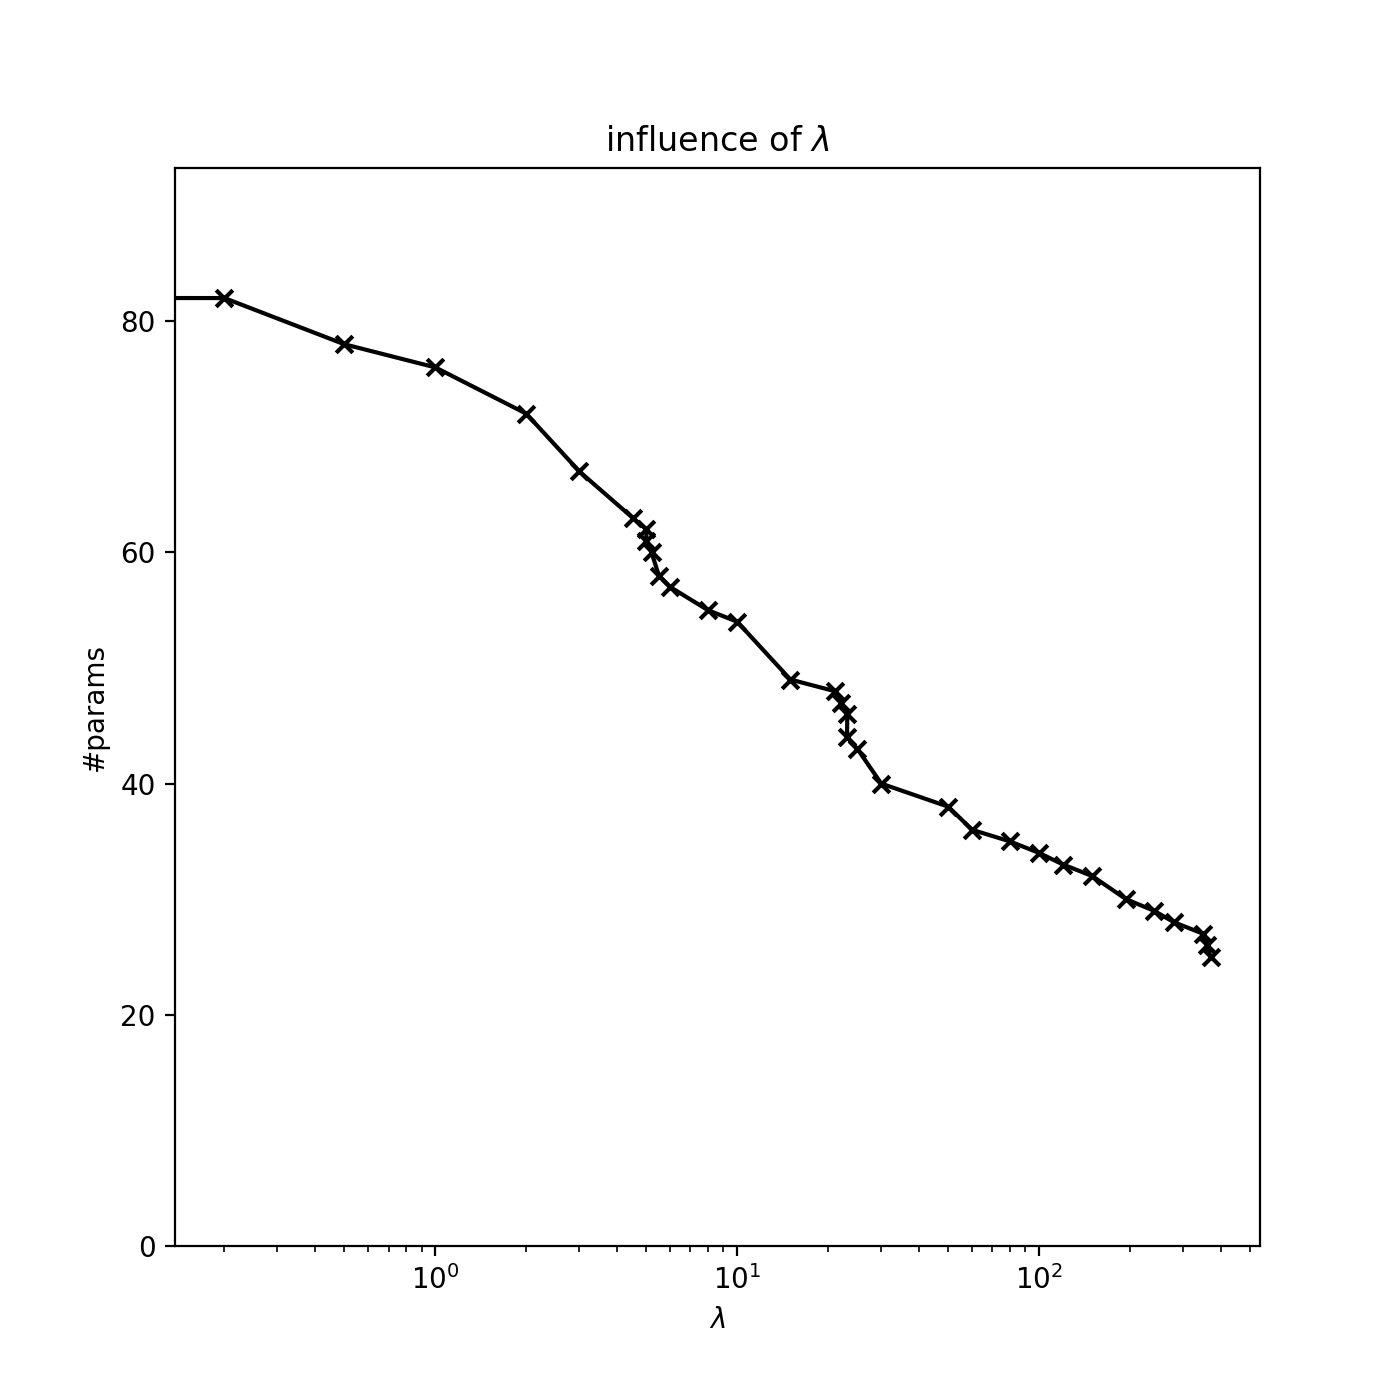
\includegraphics[scale=0.5]{graphics/n_params.png}
	\caption{Number of parameters for structures generated by different $\lambda$}
	\label{fig:results:n_params}
\end{figure}


\subsection{Parameterization}
As seen in the score history in \autoref{fig:results:parameterization}, the tabu walks are long enough to climb out of local maxima and the random restarts are short enough to not distort the adjacency matrix too much.
Sometimes the random restarts even manage to jump into better maxima (second restart in \autoref{fig:results:parameterization}).

\begin{figure}
	\centering
	\begin{subfigure}{0.2\textwidth}
		\centering
		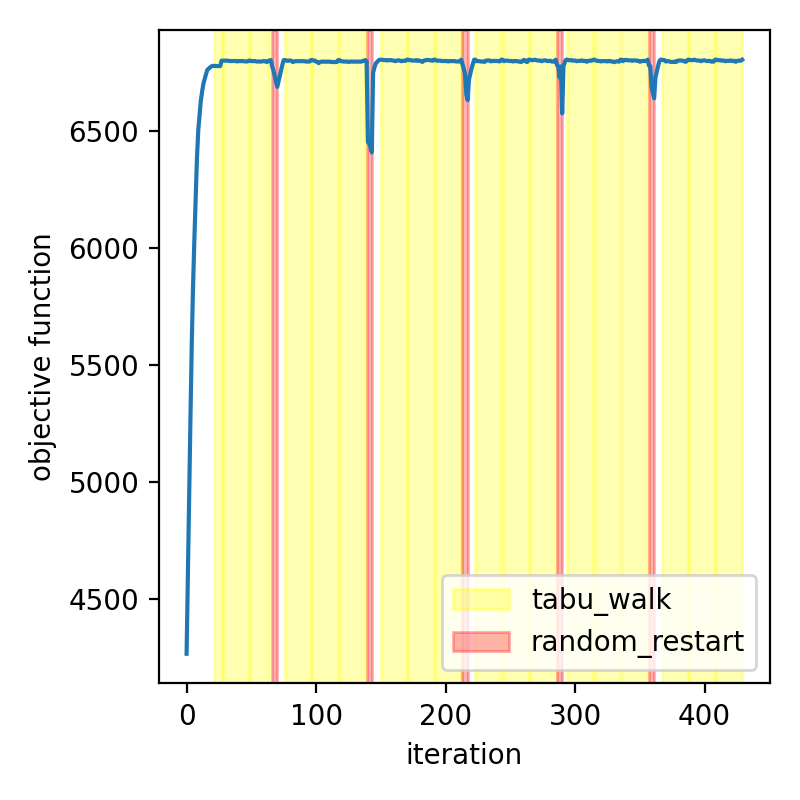
\includegraphics[scale=0.35]{graphics/scores_small_2t_2.png}
		\caption{with the first hill climb}
	\end{subfigure}
	\begin{subfigure}{0.2\textwidth}
		\centering
		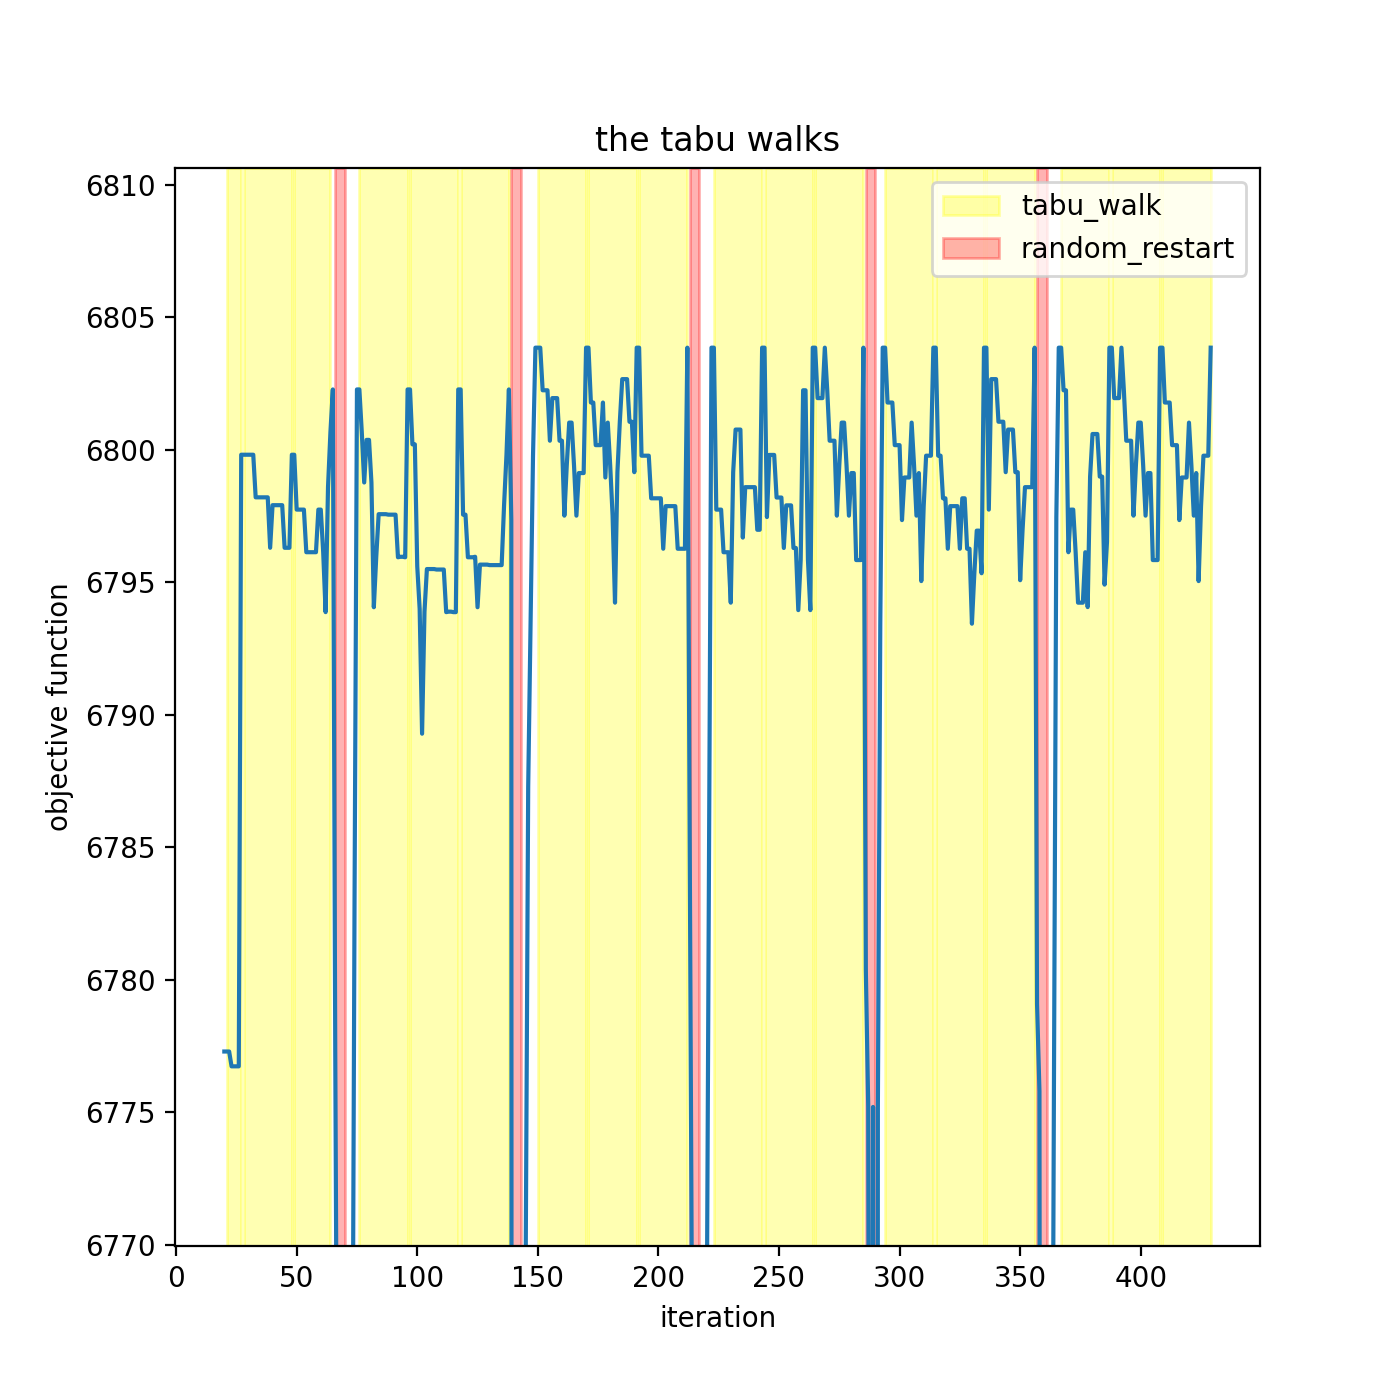
\includegraphics[scale=0.35]{graphics/tabu_small_2t_2.png}
		\caption{after the first hill climb}
	\end{subfigure}
	\caption{Score history with successful tabu walks and random restarts}
	\label{fig:results:parameterization}
\end{figure}

\subsection{Performance}
% for different lambdas, sizes of tabu walks, sizes of random walks -> include specs in appendix!
The results of the runtime measurements are illustrated in \autoref{fig:results:runtime}.
The small, medium, and big models are seperated with the red vertical lines.

\begin{figure}
	\centering
	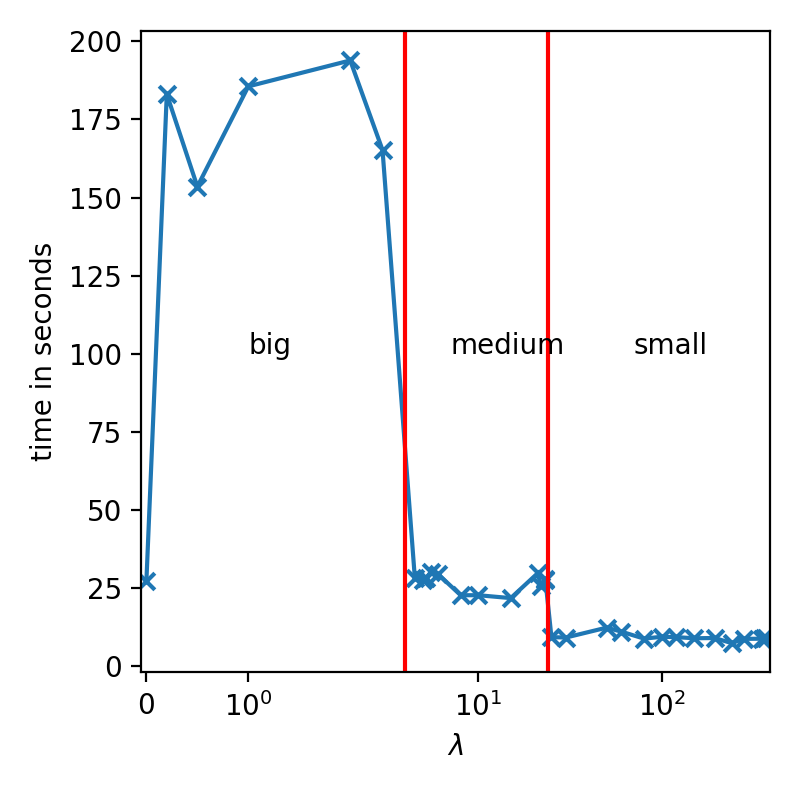
\includegraphics[scale=0.5]{graphics/times.png}
	\caption{Runtime of greedy search with different $\lambda$}
	\label{fig:results:runtime}
\end{figure}

The bigger models take much more time than the smaller models, while $\lambda$ barely has an impact.
The means that the limiting factor in the runtime of the greedy search is the length of the tabu walk.
Also for $\lambda = 0$, the runtime is strangely much shorter compared to the other big models.
The reason for this could be that a lot of possible changes improve the objective function by a very small amount after the first hill climb.
This would result in the tabu walks that are significantly shorter, which reduces the runtime.
A score history of the big model with $\lambda$ is illustrated in \autoref{fig:results:lambda_0}.
The score history confirms that the tabu walks are significantly shorter than they could be.

\begin{figure}
	\centering
	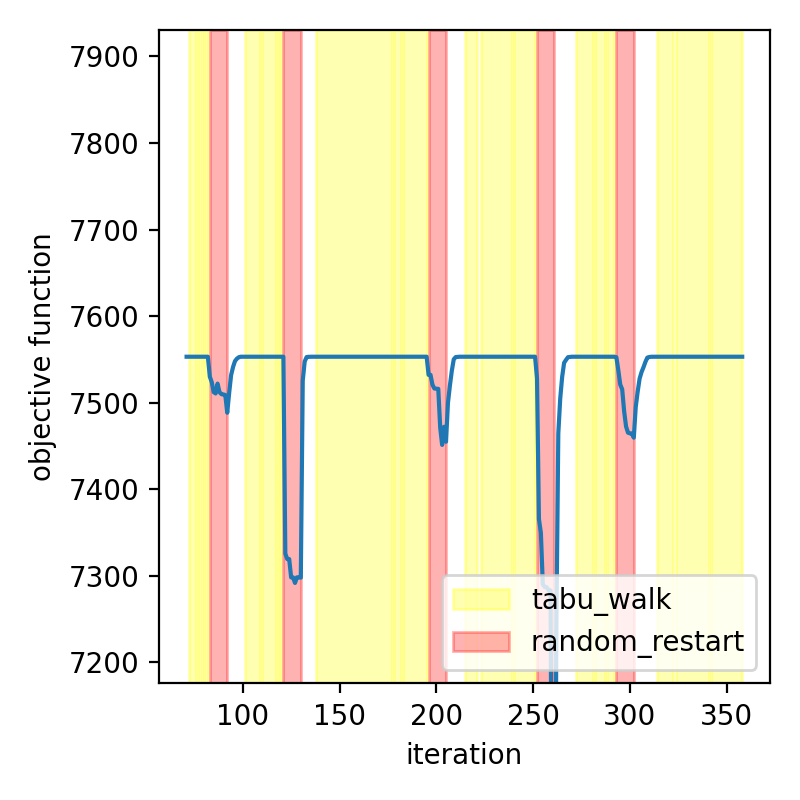
\includegraphics[scale=0.5]{graphics/tabu_lambda_0.png}
	\caption{Score history after the first hill climb, big model with $\lambda = 0$}
	\label{fig:results:lambda_0}
\end{figure}


\subsection{Likelihood}
\label{sec:results:likelihood}
The results of the likelihood measurements are illustrated in \autoref{fig:results:likelihood}.

\begin{figure}
	\centering
	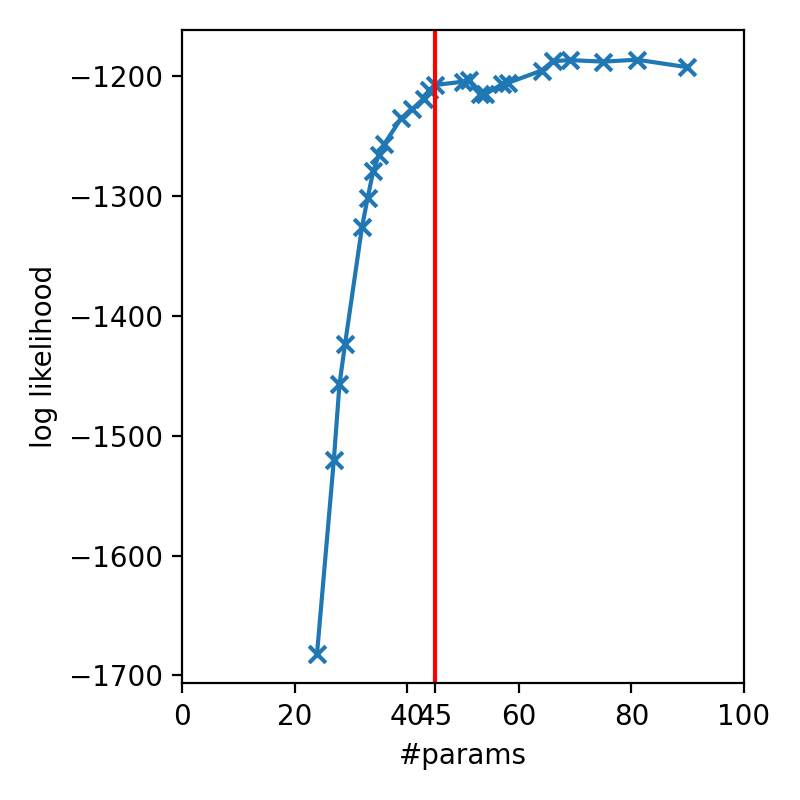
\includegraphics[scale=0.5]{graphics/likelihoods.png}
	\caption{Likelihood of adjacency matrices with different $\#params$}
	\label{fig:results:likelihood}
\end{figure}

The likelihood of the generated structures drastically increases up to $\#params = 45$.
After that, there is a small dip in likelihood and then it slowly increases again until $\#params \approx 66$ and then barely changes anymore.
Finally it reaches a likelihood that is not significantly better than at $\#params = 45$.
The reason for the small dip could be a bad parameterization of the medium sized greedy search model (see \autoref{sec:methods:analysis:parameterization}), even though it was fine-tuned the most out of the three models.

\subsubsection{Submission Scores}
% talk about how your learned structures fucking rule on the submission website we got, especially on the sparse side.
% (maybe introduce the submission website first tho - we could anonymously submit our learned structures, and they were evaluated on an secret test dataset)
The adjacency matrices i submitted to the submission website are competitive with the other top scoring adjacency matrices.
On the sparse side ($\#params \leq 33$), my adjacency matrices even hold a small, yet significant and consistent advantage over the other top scores.


\subsection{Are Longer Tabu Walks Worth It?}
In \autoref{fig:results:smaller:parameterizations} the parameterization of models for medium sized and big adjacency models are compared to the parameterization of small adjacency matrices.

\begin{figure}
	\centering
	\begin{subfigure}{0.2\textwidth}
		\centering
		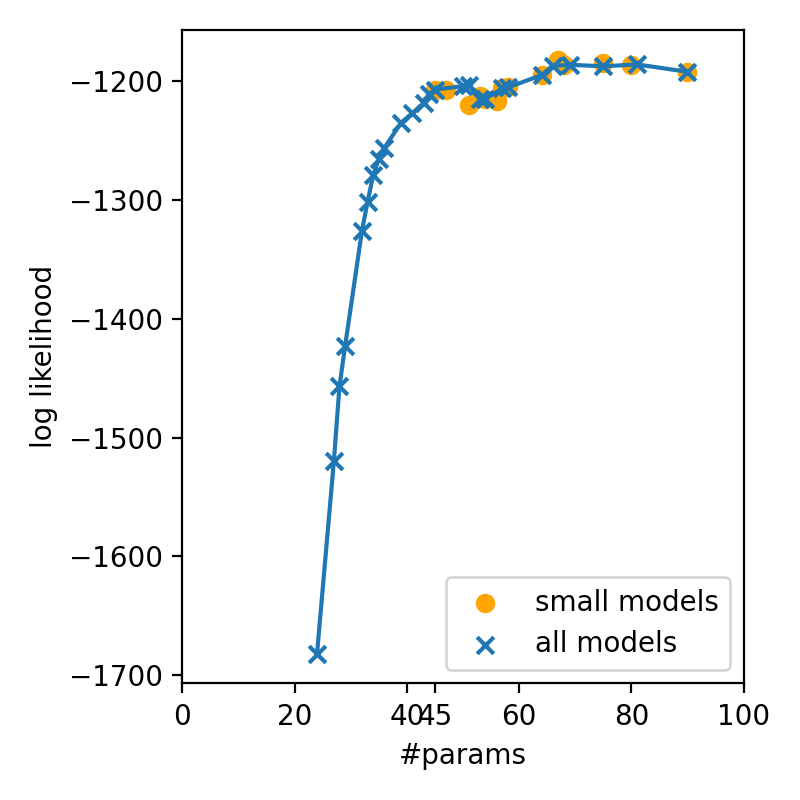
\includegraphics[scale=0.35]{graphics/both_likelihoods.png}
		\caption{Likelihood}
		\label{fig:results:smaller:likelihood}
	\end{subfigure}
	\begin{subfigure}{0.2\textwidth}
		\centering
		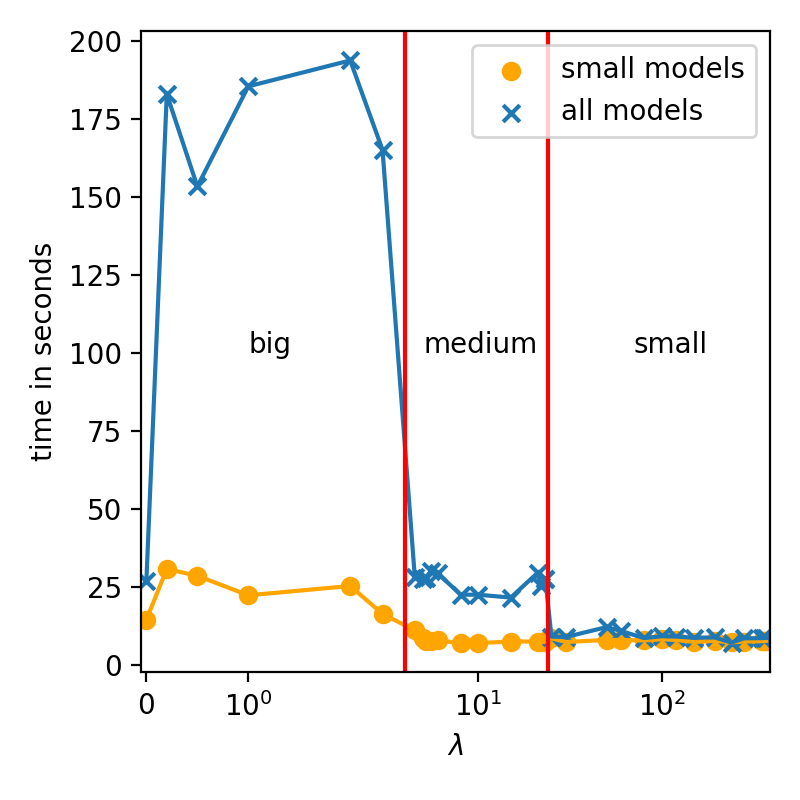
\includegraphics[scale=0.35]{graphics/both_times.png}
		\caption{Runtime}
		\label{fig:results:smaller:times}
	\end{subfigure}
	\caption{Comparison of different parameterizations}
	\label{fig:results:smaller:parameterizations}
\end{figure}

The shorter tabu walks of the small models lead to a huge improvement in runtime, and only lead to slightly worse likelihoods than medium models, and sometimes even slightly better likelihoods than the big models.
This means that the medium and big models only get slightly better results at a huge runtime cost.


\section{Conclusion}
I made an efficient, well-performing greedy search algorithm with tabu walks and random restarts.
By changing the regularization constant $\lambda$ in the objective function, the sparsity of the generated adjacency matrices can be adapted up to a very fine degree.
The greedy search performs especially well in the generation of sparse adjacency matrices.

With this greedy search, i found an adjacency matrix that is both sparse and has a high likelihood, with 45 parameters.
It is possible to get higher likelihoods with more parameters, when the tabu walks are made longer. But this comes at a cost of high runtime.

Future work could include parallelizing the search for the best performing change, finding a way to make tabu walks more efficient, and finding an efficient way of checking if a flip introduces new cycles.

\typeout{}
\bibliographystyle{ACM-Reference-Format}
\bibliography{literature}\ndy


\clearpage
\appendix
\section{Calculations}
\subsection{Score Function}
\label{sec:calc:score_function}
Here we derive
$$\max\limits_G \log p(D | G, \hat{\theta}) = \max\limits_G \sum\limits_{i \in [n]} S_i(G)$$
\begin{flalign*}
	&\max\limits_G \log p(D | G, \hat{\theta})= \max\limits_G \log \left[\prod\limits_{x \in D} p(x | G, \hat{\theta})\right]&&\\
	&= \max\limits_G \log \left[\prod\limits_{x \in D} \prod\limits_{i \in [n]} p(x_i | x_{\pa(i)}, \hat{\beta_i}, \hat{\beta_i}^*, \hat{\sigma_i})\right]&&\\
	&= \max\limits_G \sum\limits_{x \in D} \sum\limits_{i \in [n]} \log p(x_i | x_{\pa(i)}, \hat{\beta_i}, \hat{\beta_i}^*, \hat{\sigma_i})&&\\
	&= \max\limits_G \sum\limits_{x \in D} \sum\limits_{i \in [n]} \log \left[\frac{1}{\sqrt{2\pi} \sigma_i} \exp \left(-\frac{1}{2}\left(\frac{x_i - (\hat{\beta_i}^\T x_{\pa(i)} + \hat{\beta_i}^*)}{\sigma_i}\right)^2\right)\right]&&\\
	&= \max\limits_G \sum\limits_{x \in D} \sum\limits_{i \in [n]} \left[-\frac{1}{2} \left(\frac{x_i - (\hat{\beta_i}^\T x_{\pa(i)} + \hat{\beta_i}^*)}{\sigma_i}\right)^2 - \log \hat{\sigma_i} - \frac{1}{2} \log 2\pi\right]&&\\
	&= \max\limits_G \sum\limits_{i \in [n]} \underbrace{\left[-\abs{D} \cdot \log \hat{\sigma_i} - \frac{1}{2} \sum\limits_{x \in D} \left(\frac{x_i - (\hat{\beta_i}^\T x_{\pa(i)} + \hat{\beta_i}^*)}{\hat{\sigma_i}}\right)^2\right]}_{= S_i(G)}\qed&&
\end{flalign*}
Note that $\hat{\theta}$ ($\hat{\beta_i}, \hat{\sigma_i}$) depends on $G$ ($\pa(i)$).

\subsection{Graph Comparison}
\label{sec:calc:comparison}
For a graph $G'$ that was made by applying one elementary change to a graph $G$, it holds that
\begin{equation}
	\sum\limits_{i \in [n]} S_i(G') = \sum\limits_{i \in [n]} S_i(G) + \Delta_S(G', G) \label{comp_1}
\end{equation}
and
\begin{equation}
	\abs{E_{G'}} = \abs{E_{G}} + \Delta_E(G', G) \label{comp_2}
\end{equation}
Therefore
\begin{align*}
	\sum\limits_{i \in [n]} S_i(G_1) - \lambda \abs{E_{G_1}}                                  & > \sum\limits_{i \in [n]} S_i(G_2) - \lambda \abs{E_{G_2}} \\
	\stackrel{\eqref{comp_1},\eqref{comp_2}}{\iff} \Delta_S(G_1, G) - \lambda \Delta_E(G_1,G) & > \Delta_S(G_2, G) - \lambda \Delta_E(G_2,G)               \\
	\iff \Delta_S(G_1, G) - \Delta_S(G_2, G)                                                  & > \lambda \left(\Delta_E(G_1,G) - \Delta_E(G_2,G)\right)   \\
\end{align*}


\end{document}
\endinput
